\documentclass{article}
\usepackage{graphicx}
\usepackage[T1]{fontenc}
\usepackage[section]{placeins}
\usepackage[usenames,dvipsnames]{xcolor}
\usepackage{tcolorbox}
\usepackage{tabularx}
\usepackage{colortbl}
\tcbuselibrary{skins}

\tcbset{tab2/.style={enhanced,fonttitle=\bfseries,fontupper=\normalsize\sffamily,
colback=yellow!10!white,colframe=red!50!black,colbacktitle=Salmon!40!white,
coltitle=black,center title}}

\title{\textbf{\huge Dokumentacja}}

\begin{document}

\tableofcontents

\maketitle

\section{Wykorzystane technologie}
\begin{enumerate}
    \item GitHub - narzędzie do stworzenia repozytorium
    \item Quarto - narzędzie do tworzenia dokumentów naukowych i raportów (Markdown + możliwość wstawiania kodu)
    \item ERD Editor - narzędzie do stworzenia, oglądania i zmieniania schematu
    \item VisualStudioCode - edytor tekstu/kodu
    \item SQL - język zapytań użyty do tworzenia i manipulacji bazą danych
    \item MySQL - system zarządzania relacyjną bazą danych użyty do implementacji projektu
    \item Python - biblioteki {matplotlib.pyplot, numpy ,pandas, random, mysql.connector, datetime, time, timedelta, Faker}
    \item R - biblioteki {RMariaDB, kableExtra, dplyr, ggplot2, scales}
    \item Overleaf - edytor tekstu w języku Latex
\end{enumerate}

\clearpage 

\section{Struktura projektu}
\subsection{Lista plików projektu}
\begin{enumerate}
    \item create.py
    \item del.py
    \item generate.py
    \item projekt.vuerd.json
    \item raport\_bazy.pdf
    \item raport\_bazy.qmd
    \item schemat.sql
    \item Dokumentacja.pdf
    \item Dokumentacja.tex
    \item Schemat.png
\end{enumerate}
\subsection{Opis zawartości plików}\
\begin{enumerate}
    \item Tworzenie bazy danych
    \item Skasowanie bazy danych
    \item Generowanie danych
    \item Baza danych
    \item Raport w formacie .pdf
    \item Raport w formacie .qmd
    \item Schemat bazy danych 
    \item Dokumentacja w formacie pdf
    \item Tekst źródłowy dokumentacji w Latex
    \item Obrazek schematu do tekstu żródłowego Latex
\end{enumerate}


\section{Instrukcja uruchomienia projektu}
\subsection{Wymagania wstępne}
\begin{enumerate}
    \item Pobranie MySQL z https://www.mysql.com/downloads/
    \item Stwórz lokalną bazę danych.
    \item W gitbash: pip install mysql-connector-python
\end{enumerate}
\subsection{Kolejność uruchamiania plików oraz inne instrukcje}
 Połącz się do bazy danych w VisualStudioCode
\begin{enumerate}
    \item Jeśli schemat bazy danych był zmieniony to trzeba eksportować dane z pliku projekt.vuerd.json z opcją Schema SQL i nazwać go schemat.sql
    \item Uruchomić w VS po kolei create.py $\longrightarrow$ schemat.sql $\longrightarrow$ generate.py
    \item Update del.py - Jeśli masz starą wersje i chcesz ją usunąć, to trzeba ponownie prześć do punktu 2. żeby stworzyć baze i wgrać nowe dane
\end{enumerate}

\section{Projekt bazy danych}
\subsection{Schemat bazy danych}
\begin{figure}[!htb]
    \caption{Schemat}
    \centering
  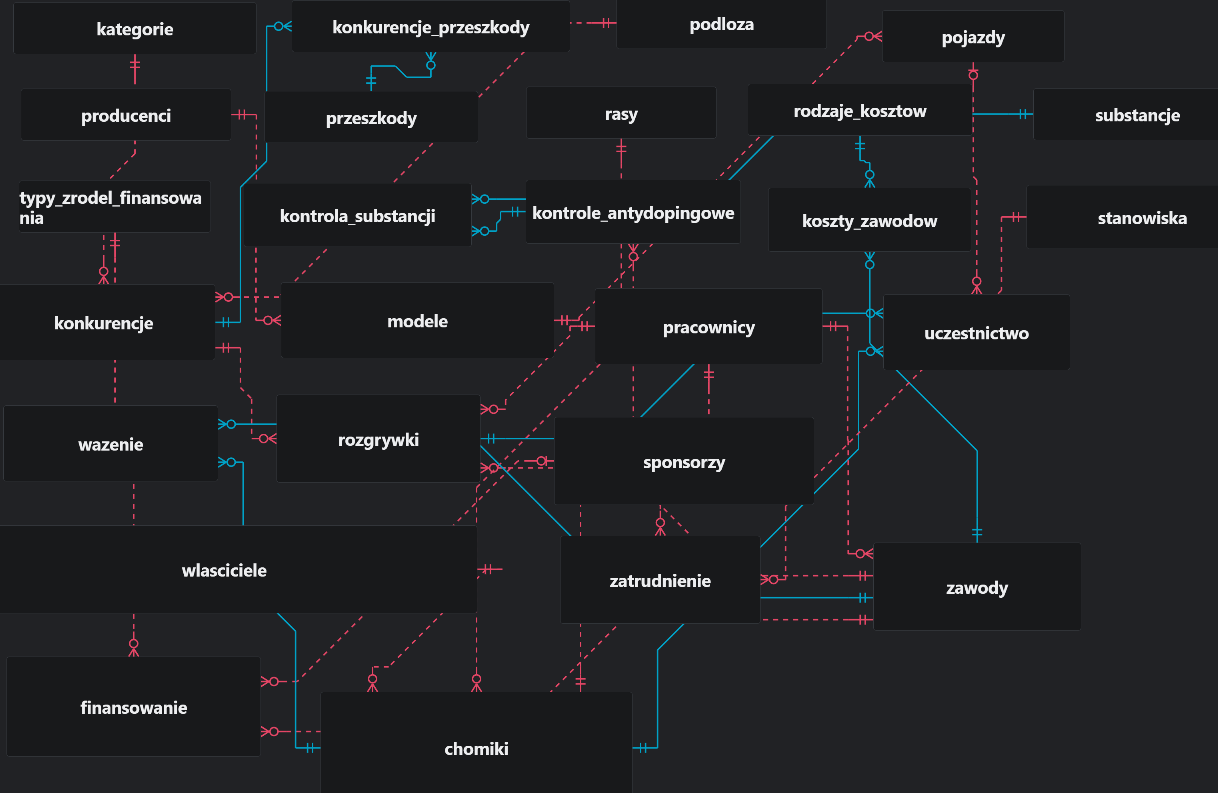
\includegraphics[width=1\textwidth]{Schemat.png}
    \label{fig7}
\end{figure}

\clearpage

\subsection{Relacje}
\begin{enumerate}
    \item konkurencje $\longrightarrow$ kategorie poprzez klucz id\_kategorii
    \item modele $\longrightarrow$ producenci poprzez klucz id\_producenta
    \item finansowanie $\longrightarrow$ typy\_zrodel\_finansowania poprzez klucz id\_typu
    \item konkurencje\_przeszkody $\longrightarrow$ konkurencje poprzez klucz id\_konkurencji
    \item rozgrywki $\longrightarrow$ konkurencje poprzez klucz id\_wlasciciela
    \item konkurencje\_przeszkody $\longrightarrow$ przeszkody poprzez klucz id\_przeszkody
    \item pojazdy $\longrightarrow$ modele poprzez klucz id\_modelu
    \item uczestnictwo $\longrightarrow$ rozgrywki poprzez klucz id\_rozgrywki
    \item wazenie $\longrightarrow$ chomiki poprzez klucz id\_chomika
    \item kontrole\_antydopingowe $\longrightarrow$ chomiki poprzez klucz id\_chomika
    \item uczestnictwo $\longrightarrow$ chomiki poprzez klucz id\_chomika
    \item chomiki $\longrightarrow$ rasy poprzez klucz id\_podloza
    \item kontrola\_substancji  $\longrightarrow$ kontrole\_antydopingowe poprzez klucz id\_kontroli
    \item rozgrywki $\longrightarrow$ pracownicy poprzez klucz id\_pracownika
    \item zatrudnienie $\longrightarrow$ pracownicy poprzez klucz id\_pracownika
    \item zawody $\longrightarrow$ pracownicy poprzez klucz id\_pracownika
    \item finansowanie $\longrightarrow$ sponsorzy poprzez klucz id\_firmy
    \item konkurencje $\longrightarrow$ podloza poprzez klucz id\_rasy
    \item koszty\_zawodow $\longrightarrow$ rodzaje\_kosztow poprzez klucz id\_kosztu
    \item finansowanie $\longrightarrow$ zawody poprzez klucz id\_zawodow
    \item wazenie $\longrightarrow$ zawody poprzez klucz id\_zawodow
    \item rozgrywki $\longrightarrow$ zawody poprzez klucz id\_zawodow
    \item koszty\_zawodow $\longrightarrow$ zawody poprzez klucz id\_zawodow
    \item kontrola\_substancji $\longrightarrow$ substancje poprzez klucz id\_substancji
    \item zatrudnienie $\longrightarrow$ stanowiska poprzez klucz id\_stanowiska
    \item uczestnictwo $\longrightarrow$ pojazdy poprzez klucz id\_pojazdu
\end{enumerate}

\section{Analiza zależności funkcyjnych}
\subsection{Tabela - kategorie}

\begin{tcolorbox}[tab2,tabularx={X||X|X}]
Zależność funkcyjna & Wyjaśnienie     \\
\hline
\hline
id\_kategorii → nazwa\_kategorii & Każda kategoria ma jedną nazwę \\    
\end{tcolorbox}

\subsection{Tabela - producenci}

\begin{tcolorbox}[tab2,tabularx={X||X}]
Zależność funkcyjna & Wyjaśnienie     \\
\hline
\hline
id\_producenta → nazwa\_producenta & Każdy producent ma jedną nazwę \\     
\end{tcolorbox}

\subsection{Tabela - typy\_zrodel\_finansowania}

\begin{tcolorbox}[tab2,tabularx={X||X}]
Zależność funkcyjna & Wyjaśnienie     \\
\hline
\hline
id\_typu → nazwa\_typu) & Każdy typ ma jedną nazwę \\    
\end{tcolorbox}

\subsection{Tabela - finansowanie}

\begin{tcolorbox}[tab2,tabularx={X||X}]
Zależność funkcyjna & Wyjaśnienie     \\
\hline
\hline
(id\_finansowania, id\_zawodow, id\_typu, id\_firmy) → (data\_wyplaty, kwota) & Data wypłaty przypisana do odpowiedniego finansowania, zawodów, typu oraz firmy \\    
\end{tcolorbox}

\subsection{Tabela - konkurencje}

\begin{tcolorbox}[tab2,tabularx={X||X}]
Zależność funkcyjna & Wyjaśnienie     \\
\hline
\hline
(id\_kategorii, id\_konkurencji, id\_podloza) → dlugosc\_trasy & Długość przypisana do konkretnej kategorii, konkurencji i podłoża \\  \\    
\end{tcolorbox}

\subsection{Tabela - wazenie}

\begin{tcolorbox}[tab2,tabularx={X||X}]
Zależność funkcyjna & Wyjaśnienie     \\
\hline
\hline
(id\_chomika, id\_zawodow) → (waga, data\_wazenia) & Waga oraz data ważenia przypisane do odpowiedniego chomika oraz zawodów\\  \\    
\end{tcolorbox}

\subsection{Tabela - wlasciciele}

\begin{tcolorbox}[tab2,tabularx={X||X}]
Zależność funkcyjna & Wyjaśnienie     \\
\hline
\hline
id\_wlasciciela → (imie\_walsciciela, nazwisko\_wlasciciela, numer\_telefonu, zodiak\_wlasciciela) & Imię, nazwisko, numer telefonu oraz zodiak przypisany do odpowiedniego właściciela \\  \\    
\end{tcolorbox}

\subsection{Tabela - przeszkody}

\begin{tcolorbox}[tab2,tabularx={X||X}]
Zależność funkcyjna & Wyjaśnienie     \\
\hline
\hline
id\_przeszkody → rodzaj\_przeszkody & Rodzaj przeszkody przypisany do odpowiedniej przeszkody \\  \\    
\end{tcolorbox}

\subsection{Tabela - kontrola\_substancji}

\begin{tcolorbox}[tab2,tabularx={X||X}]
Zależność funkcyjna & Wyjaśnienie     \\
\hline
\hline
(id\_kontroli, id\_substancji) → wynik\_testu & Wynik testu przypisany do odpowiedniej substancji oraz kontroli \\  \\    
\end{tcolorbox}

\subsection{Tabela - modele}

\begin{tcolorbox}[tab2,tabularx={X||X}]
Zależność funkcyjna & Wyjaśnienie     \\
\hline
\hline
(id\_producenta, id\_modelu) → (nazwa\_modelu, cena\_modelu) & Nazwa i cena modelu przypisana do odpowiedniego modelu i pruducenta \\ 
\end{tcolorbox}

\subsection{Tabela - rozgrywki}

\begin{tcolorbox}[tab2,tabularx={X||X}]
Zależność funkcyjna & Wyjaśnienie     \\
\hline
\hline
(id\_rozgrywki, id\_zawodow, id\_konkurencji, id\_sedzi) → data\_rozgrywki & Data rozgrywki przypisana do odpowiedniej rozgrywki, zawodów, konkurencji oraz sędziego\\  \\    
\end{tcolorbox}

\subsection{Tabela - chomiki}

\begin{tcolorbox}[tab2,tabularx={X||X}]
Zależność funkcyjna & Wyjaśnienie     \\
\hline
\hline
(id\_chomika, id\_wlasciciela, id\_rasy) → (imie\_chomika, data\_urodzenia, data\_dolaczenia, data\_odejscia) & Imię, data urodzenia, data dołączenia oraz data odejścia przypisana do odpowiedniego chomika, właściciela oraz rasy chomika \\  \\    
\end{tcolorbox}

\subsection{Tabela - rasy}

\begin{tcolorbox}[tab2,tabularx={X||X}]
Zależność funkcyjna & Wyjaśnienie     \\
\hline
\hline
id\_rasy → nazwa\_rasy & Każda rasa ma jedną nazwę \\  \\    
\end{tcolorbox}

\subsection{Tabela - kontrole\_antydoppingowe}

\begin{tcolorbox}[tab2,tabularx={X||X}]
Zależność funkcyjna & Wyjaśnienie     \\
\hline
\hline
(id\_kontroli, id\_chomika) → data\_kontroli & Data przypisana do odpowiedniej kontrolii oraz chomika \\  \\    
\end{tcolorbox}

\subsection{Tabela - pracownicy}

\begin{tcolorbox}[tab2,tabularx={X||X}]
Zależność funkcyjna & Wyjaśnienie     \\
\hline
\hline
id\_pracownika → (imie\_pracownika, nazwisko\_pracownika, numer\_telefonu) & Imię, nazwisko, numer telefonu przypisane do odpowiedniego pracownika \\  \\    
\end{tcolorbox}

\subsection{Tabela - sponsorzy}

\begin{tcolorbox}[tab2,tabularx={X||X}]
Zależność funkcyjna & Wyjaśnienie     \\
\hline
\hline
id\_firmy → (nazwa\_firmy, dane\_kontaktowe, rozpoczecie\_wspolpracy, zakonczenie\_wspolpracy) & nazwa, dane kontaktowe firmy oraz rozpoczęcie i zakończenie współpracy dla odpowiedniej firmy\\  \\    
\end{tcolorbox}

\subsection{Tabela - zatrudnienie}

\begin{tcolorbox}[tab2,tabularx={X||X}]
Zależność funkcyjna & Wyjaśnienie     \\
\hline
\hline
(id\_zatrudnienia, id\_stanowiska, id\_pracownika) → (data\_zatrudnienia, data\_zwolnienia) & Data zatrudnienia i zwolnienia przypisana do odpowiedniego zatrudnienia i stanowiska pewnego pracownika \\  \\    
\end{tcolorbox}

\subsection{Tabela - podloza}

\begin{tcolorbox}[tab2,tabularx={X||X}]
Zależność funkcyjna & Wyjaśnienie     \\
\hline
\hline
id\_podloza → nazwa\_podloza & Każde podłoże ma jedną nazwę \\  \\    
\end{tcolorbox}

\subsection{Tabela - rodzaje\_kosztow}

\begin{tcolorbox}[tab2,tabularx={X||X}]
Zależność funkcyjna & Wyjaśnienie     \\
\hline
\hline
id\_kosztu → nazwa\_kosztu & Każdy koszt ma jedną nazwę ze zbioru słów {wynajem, nagrody, itp.} \\  \\    
\end{tcolorbox}

\subsection{Tabela - koszty\_zawodow}

\begin{tcolorbox}[tab2,tabularx={X||X}]
Zależność funkcyjna & Wyjaśnienie     \\
\hline
\hline
(id\_zawodow, id\_typy\_kosztu) → kwota & Kwota przypisana doodpowiednich zawodów oraz typu kosztu \\  \\    
\end{tcolorbox}

\subsection{Tabela - uczestnictwo}

\begin{tcolorbox}[tab2,tabularx={X||X}]
Zależność funkcyjna & Wyjaśnienie     \\
\hline
\hline
(id\_chomika, id\_rozgrywki, id\_pojazdu) → miejsce & Miejsce przypisane do odpowiedniego chomika, rozgrywki oraz pojazdu \\  \\    
\end{tcolorbox}

\subsection{Tabela - zawody}

\begin{tcolorbox}[tab2,tabularx={X||X}]
Zależność funkcyjna & Wyjaśnienie     \\
\hline
\hline
(id\_zawodow, id\_koordynatora) → (data\_rozpoczecia, data\_zakonczenia, liczba\_widzow) & Data rozpoczęcia i zakończenia oraz liczba widzów dla odpowiednich zawodów oraz koordynatora \\  \\    
\end{tcolorbox}

\subsection{Tabela - substancje}

\begin{tcolorbox}[tab2,tabularx={X||X}]
Zależność funkcyjna & Wyjaśnienie     \\
\hline
\hline
id_substancji → nazwa_substacji & Każda substancja ma jedną nazwę \\  \\    
\end{tcolorbox}

\subsection{Tabela - stanowiska}

\begin{tcolorbox}[tab2,tabularx={X||X}]
Zależność funkcyjna & Wyjaśnienie     \\
\hline
\hline
id\_stanowiska → (nazwa\_stanowiska, wyplata) & Wypłata oraz nazwa stanowiska dla odpowiedniego stanowiska \\  \\    
\end{tcolorbox}

\section{Normalizacja bazy danych}
\subsection{Uzasadnienie spełnienia EKNF}
Baza danych została zaprojektowana zgodnie z zasadami EKNF.
We wszystkich relacjach jedynymi nietrywialnymi zależnościami funkcyjnymi są zależności,
w których lewa strona stanowi klucz główny danej relacji.
W bazie nie występują zależności częściowe ani przechodnie pomiędzy atrybutami niekluczowymi.
Każda relacja spełnia więc warunek EKNF.

\section{Problemy napotkane podczas realizacji projektu}
Największym wyzwaniem było zrobienie schematu zgodnego z EKNF.

\end{document}
